\subsection{Load-step}
Load-steppet er i 3. iteration simuleret på samme måde, som det blev gjort under 2. iteration i sektion ~\ref{loadstep2ite}. Med en større båndbredde ændrer systemets loadstep. Derfor ser loadsteppet efter de nye gain-phase målinger ud som på ~\ref{fig:Loadstepsim2}
\begin{figure}[H]
	\center
	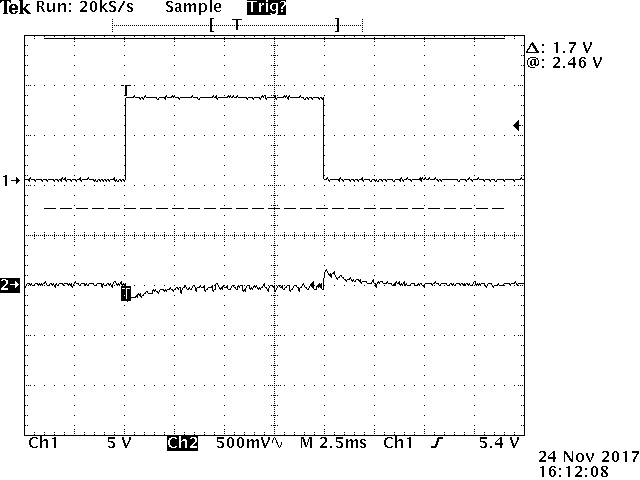
\includegraphics[max width=0.7\linewidth]{/tex/3iteration/billeder/simulering/Loadstep.PNG}
	\caption{Realiseret load-step}
	\label{fig:Loadstepsim2}
\end{figure} 
Her ses det, at overshootet er blevet mindre. Det aflæses til ca. $300mV$ ved første dyk og $200mV$ ved stigningen. Selve reguleringstiden er blevet noget længere og aflæses til ca. $4ms$ for begge loads. 
